%%%%%%%%%%%%%%%%%%%%%%%%%
%%
%% $Author: Deepti Hegde $
%% $Datum: 2023-06-25  $
%% $Pfad: BA23-02-Sales-Predictor/report/Contents/en/Introduction.tex $
%% $Version: 1.0 $
%% $Reviewed by: Deepti, Sadegh and Raunak $
%% $Review Date: 2023-06-30 $
%%
%%%%%%%%%%%%%%%%%%%%%%%%%
%
%\chapter{Documentation Developer} 
%
%\section{Structure and Idea}
%
%	The purpose of this report is to outline the process of developing a sales prediction model using the XGBoost algorithm. This chapter provides an overview of the documentation structure, the idea behind the project, the flowchart of the implementation, and the machine learning pipeline employed.
%	
%	The documentation for this sales prediction project follows a structured approach to ensure clarity and ease of understanding. It provides a brief overview of the project's objective and contents of the report. Describes the process of acquiring and preparing the dataset for analysis. In addition to that, explains the techniques used and the steps involved in training and evaluating the XGBoost model.
%	
%	The main \textbf{idea} of this project is to create a machine learning model that can predict sales reliably based on previous data and pertinent attributes. We intend to construct a robust and reliable sales prediction model by leveraging the XGBoost algorithm, which is well-known for its ability in dealing with structured data and gradient boosting.
%	
%	\subsection{Flow chart}
%		
%		The flow chart below illustrates the high-level process of developing the sales prediction model using XGBoost starting from data collection to model evaluation.
%		
%		\begin{center}
%			\begin{figure}[h!]
%				\begin{center}
%					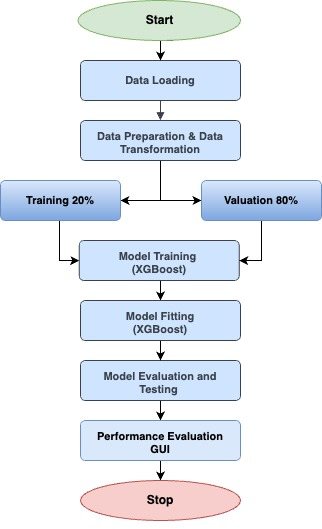
\includegraphics[height=125mm, width=130mm]{Images/DevelopmentFlowChart}
%				\end{center}
%				\caption{ XGBoost Development FlowChart}
%			\end{figure}
%		\end{center}
%
%
%	\subsection{ML Pipeline}
%	
%	\begin{itemize}
%		
%		\item Data Collection: 
%		
%		Collect historical sales data, including important elements such as product information, time series data, and external factors that may influence sales.
%		
%		\item Data Preprocessing: 
%		
%		Remove missing values, outliers, and formatting errors from the data. If necessary, perform feature scaling or normalization.
%		
%		\item Feature Engineering: 
%		
%		Use techniques such as one-hot encoding, feature extraction, or establishing lag variables to transform raw data into meaningful features.
%		
%		\item Model Training: 
%		
%		Train the XGBoost model using the training set. This involves fitting the model to the training data and optimizing the model's hyperparameters to find the best combination for your specific problem. The XGBoost algorithm utilizes gradient boosting to iteratively improve the model's predictions.
%		
%		\item Model Evaluation: 
%		
%		Use appropriate evaluation measures to assess the model's performance, such as mean squared error (MSE), root mean squared error (RMSE), or R-squared value. If necessary, fine-tune the model.
%		
%		\item Prediction: 
%		
%		Deploy the trained model to make predictions on new, unseen data to estimate future sales.
%		
%	\end{itemize}
%	
%		\begin{center}
%		\begin{figure}[h!]
%			\begin{center}
%				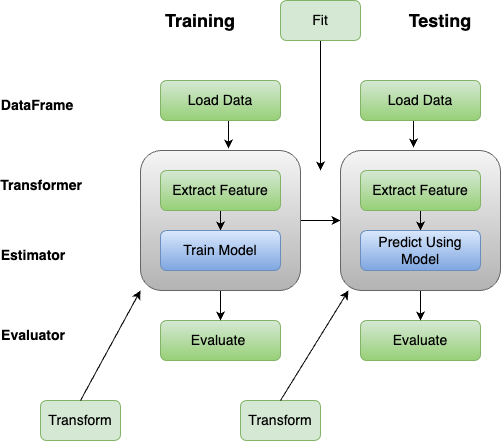
\includegraphics[height=90mm, width=130mm]{Images/MLPipeline}
%			\end{center}
%			\caption{ ML Pipeline for Sales Prediction}
%		\end{figure}
%	\end{center}